\section{Resultate}\label{resultate}
Wie im Kapitel \ref{konzept} wird erwähnt, dass der Ist-Zustand die Feldlinien im FITS-Dateiformat abspeichert. Es wurde geprüft, wie viel Speicher das Format nach der Entropie-Kodierung beansprucht. Für den Test wurde die Komprimierung \ref{resultate:loesung0} werwendet und die Daten im FITS-Dateiformat und als Binärdatei abgelegt.
figure
Die Resultate \ref{} zeigen keinen signifikanten Unterschied des Speicherverbrauchs. Pro Feldlinie liegt der Unterschied bei einem Byte. Hochgerechnet sind es 1.2 KiBytes, welches das Fits-Format für sich beansprucht. Ein Teil der 1.2KiBytes sind vermutlich die String-Namen der Datenreihen. Fits erlaubt es, den Datenreihen einen Namen so wie eine kurze Beschreibung anzuhänken.

\subsection{Lösung 0, Angle-Subsampling} \label{resultate:loesung0}
Das Angle-Subsampling führt der JHelioviewer selbst durch. Für die Lösung 0 soll nun das Subsampling vor der Dateiübertragung vorgenommen werden. Dazu werden die Punkte in das kartesische Koordinatensystem umgerechnet, das Angle-Subsampling durchgeführt und anschliessend wird in das sphärische System rücktransformiert. Die resultierende FITS-Datei wird mittels Rar kodiert.
\begin{figure}[!htbp]
	\center
	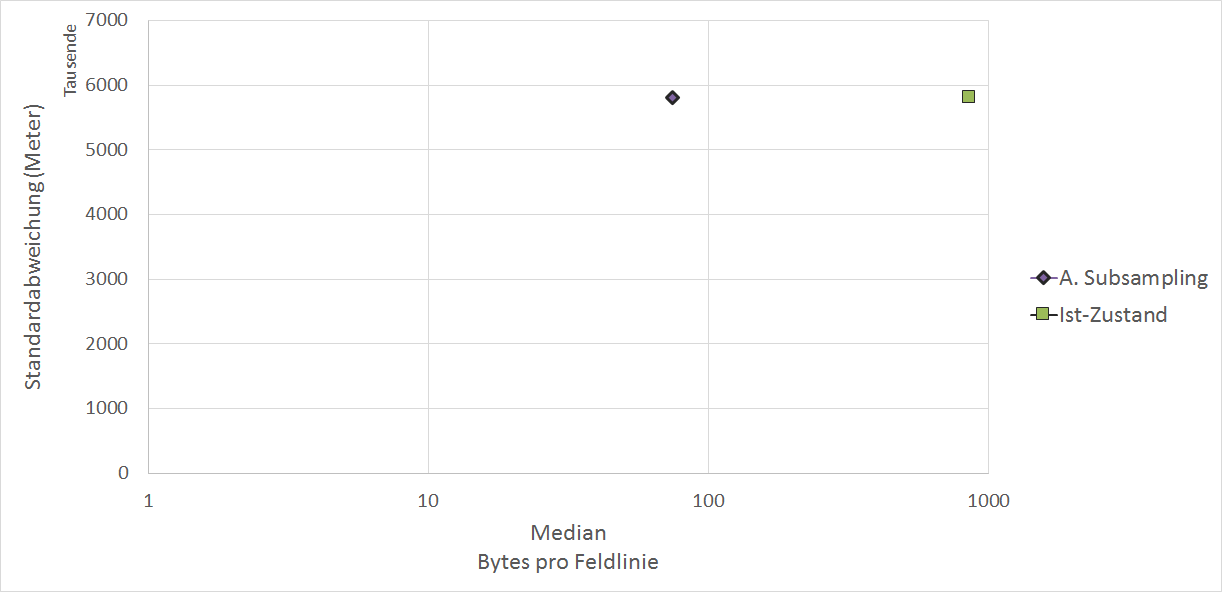
\includegraphics[width=0.8\textwidth,height=6cm,keepaspectratio]{./pictures/resultate/loesung0/loesung0_0.png}
	\caption{Vergleich der Lösung 0 zum Ist-Zustand.}
	\label{resultate:loesung0:loesung0_0}
\end{figure}
Wie im Diagramm \ref{resultate:loesung0:loesung0_0} erkennbar ist, verbraucht die Lösung 0 um grössenordnungen weniger Speicher. Zu einem wird durch das Angle-Subsampling weniger Daten gespeichert,etwa nur ein Viertel der ursprünglichen Punkte. Zum anderen erbringt Rar die bessere Kompression. Die Komplexität der Kompression und Dekompression bleibt in der Grössenordnung $O(n)$ ($n$ ist die Anzahl Punkte). Da bei der Dekompression $n$ etwa vier Mal weniger Punkte bearbeiten muss, ist die Dekompression sogar schneller als die Ist-Lösung.

\subsubsection{Variante PCA}
Durch die PCA könnte die Komprimierung weiter verbessert werden. Die unterschiedliche Orientierung der Feldlinien spielen keine Rolle mehr und die Chance ist höher, dass zwei Feldlinien ähnliche Punkte aufweisen. Dadurch könnte die Entropie-Kodierung eine bessere Kompression erzeugen.
Kartesische Koordinaten, Subsampling, 
figure
Leider nicht, es liegt zu einen an den Daten, welche zusätzlich gespeichert werden, 6 floats für das neuen koordinatenachsen und 3 floats für den Durchschnitt

\subsubsection{Artefakte}

\subsection{Lösung 1, Diskrete Kosinus Transformation}
Das Ziel ist eine bessere Kompression zu erreichen, indem die Feldlinien mit Kosinusfunktionen approximiert werden. 
Die DCT-Implementierung für die Tests weist eine Komplexität von $O(n^2)$. Bei etwa $600$ Punke pro Linie ist das zu erheblichen Rechenaufwand. Deshalb wird vor der DCT deshalb ein Subsampling durch. Falls die Laufzeit der Dekompression verbessert werden soll, kann die Fast-Cosine-Transformation umgesetzt werden. Diese hat eine Komplexität von $O(n log n)$. Falls das nicht ausreicht, können die Linien in Blöcken mit einer bestimmten Anzahl von Punkten unterteilt werden. Das senkt die Komplexität auf $O(n)$. Aber die Unterteilung könnte negative Effekte auf die Kompression haben.\\
[\baselineskip]
In den Tests wurde eine lineare Quantisierung verwendet. Jeder DCT Koeffizient wird durch einen Faktor geteilt, der sich stetig ehöht. Zum Beispiel wird der erste Koeffizient durch zwei geteilt, der zweite durch Vier, der Dritte durch Sechse etc.  Die Kompressionsrate kann durch einen höheren oder tieferen Faktor gesteuert werden. Diese Quantifizierung ist nicht das Optimum. Eine bessere Quantifizierung wird für die beste Lösung ausgearbeitet.

\subsubsection{DCT}
Nach dem Subsampling wird auf den Punkten (im kartesischen Koordinatensystem) die Diskrete Kosinus Transformation ausgeführt. Es ist auch möglich die Punkte im sphärischen Koordinatensystem in den Frequenzraum zu überführen. Der $\phi$-Kanal ist jedoch schwierig durch tiefe Kosinus schwingungen darzustellen: Wie im Abschnitt \ref{konzept:ist-komprimierung} besprochen, beinhaltet der Kanal Sprünge bei der Passierung des Nullpunktes. Das führt zu sehr hochfrequenten Schwingungsanteile in der DCT. Nach einer Quantisierung sind dabei Artefakte nicht vermeidbar. Im kartesischen System hingegen sind alle Kanäle stetig haben somit weniger hochfrequente Anteile.\\
Die Anzahl Punkte pro Linie werden zuerst als Short-Array abgelegt, gefolgt von allen DCT Koeffizienten des X Kanals, danach des Y und zum Schluss des Z Kanals
(Figure)
Lösung leicht besser als die Lösung 0, der Maximale Fehler ist aber überproportional gross.
(Artefakte)
Hochfrequente Anteile werden nicht dargestellt, was in diesem Fall bedeutet, dass hohe Steigungen nicht dargestellt werden können. Die Form kann also nicht gehalten werden.

\subsubsection{Angle-Subsampling mit DCT}
Nicht vielversprechend, da sehr hohe Varianz in den Daten, aber Angle-Subsampling wirft sehr viele Daten weg.
figure 
wie man sehen kann, klappt es nicht. Der Fehler schiesst in die Höhe

\subsubsection{Feldlinien Ableiten mit DCT}\label{resultate:dct:ableitung_dct}
Ziel der Ableitung: Weniger grosse Zahlen, dämpfung des DC-Koeffizienten. Hochfrequente Anteile sind jetzt hohe veränderungen in den Kurven. Dafür wird die Kurve immer Ungenauer.
Umsetzung der ableitung
DA alles viel kleiner ist, können die 
figure vergleich Lösung1 und 1-1
Kann gut Quantisiert werden, es kann der Grossteil der DCT Komponenten auf 0 gesetzt werden. 
(Vergleich der Artefakte).
Stellt die Kurven um einiges besser dar.\\
[\baselineskip] Rar scheint allgemein einfacher Integers komprimieren zu können.

\subsubsection{Feldlinien Ableiten mit PCA und DCT}
Selbe Idee wie in \ref{resultate:dct:ableitung_dct}, nur jetzt mit einer Principal Component analysis. Erhofft sich zu einem bessere Quantisierung, da oft ein Kanal fast wegfällt und zum anderen eine bessere Entropie kodierung, da es jetzt sein kann dass ähnliche Kurven auch ähnliche DCT Parameter aufweisen. Der Nachteil ist, dass für die Rücktransformation pro linie neue Information gespeichert werden muss.
figure Vergleich 1-1 und 1-4
Der Aufwand lohnt sich nicht, obwohl die PCA vielversprechend scheint. Feldlinien liegen ungefähr in einer Ebene. Dadurch kaum noch etwas im Z-kanal, fast alles 0.
DCTKoeffizientenvergleich
X Kanal allgemein grösser, aber y und z kanal tiefer. Schlussendlich scheint die PCA keinen signifikanten Vorteil zu bringen.


\subsubsection{Artefakte}
2D Feldlinie zeigen, normal und komprimiert
